%%==================================================================
\section{Further worked applications}\label{sec:more}\enlargethispage{4pt}
%%==================================================================

The applications of Section~\ref{sec:applications} used one Boolean variable
per vertex or per clause variable, one algebra generator, and constraints of the
simplest kind. This section works out eight further families in which one of
these three choices is made differently: several generators record several
linear statistics at once; the variables range over a finite domain and the
objective is a cut into several classes; the variables sit on the edges of a
bounded-degree graph and the constraints at the vertices; the algebra is $\Q$
but the factor is the Fortuin--Kasteleyn weight of an edge, which reaches the
Tutte polynomial on a hyperbola; the constraints are the parity checks of a
linear code; the constraints are the incidences of a hypergraph; the
constraints are the gates of a circuit; and the constraints are the rows of
an integer program, linear inequalities with coefficients of arbitrary size. In each case the proof consists of
naming the variables, the factors and the algebra, checking the three
hypotheses of Theorem~\ref{thm:weighted} or Theorem~\ref{thm:domain}, and
reading the answer off the resulting element of the algebra. We use throughout
that $\rhon$ is increasing on $[20,\infty)$,\footnote{With $u=\log x$ and
$u'=1/(x\ln 2)$ the logarithmic derivative of $\rhon(x)=x(\log u)^2/\sqrt u$ is
$1/x+2u'/(u\ln 2\,\log u)-u'/(2u)$, and the negative term is at most
$1/(2x\,u\ln 2)<1/x$ for $u\ge 1$.} so that $\rhon(m)\le\rhon(Cn)\le 4C\rhon(n)$
whenever $20\le m\le Cn$ and $n\ge C$, as in the proof of
Theorem~\ref{thm:domain}.

\subsection{Several linear side constraints}\label{ssec:linear}
Corollary~\ref{cor:hamming} and Proposition~\ref{prop:modular} recorded one
linear statistic of the assignment in the exponent of the single generator $W$.
With the algebra $\A_{N_1,\dots,N_s}$ of \eqref{eq:ANs} one records $s$ of them
at once, and a fixed number of linear equations or congruences may be imposed
on the solutions of a sparse constraint system.

\begin{theorem}[Linear statistics]\label{thm:linear}
Fix integers $k,c,s\ge1$. Let $(\Phi_f)_{f\in\F}$ be a factor system on $n\ge20$
Boolean variables with at most $cn$ factors of scope at most $k$, with values in
$\A_{N_0}$ for some $N_0\ge1$ and coefficients that are polynomials in $W_0$ with
integer coefficients of at most $L$ bits, and let
$\omega^{(1)},\dots,\omega^{(s)}\in\{0,1,\dots,\Omega\}^n$ be weight vectors.
\begin{enumerate}[label=\textup{(\roman*)},leftmargin=2.2em]
\item\label{it:lineq} The elements
\[
  r(j_1,\dots,j_s)=\sum_{x\in\{0,1\}^n:\ \sum_v\omega^{(i)}_vx_v=j_i\ (1\le i\le s)}
  \ \prod_{f\in\F}\Phi_f(x)\ \in\A_{N_0}
\]
are computed, for all $(j_1,\dots,j_s)$ at once, in time
$\poly\bigl(n,L,N_0,(1+n\Omega)^s\bigr)2^{O_{k,c}(\rhon(n))}$.
\item\label{it:lincong} For moduli $M_1,\dots,M_s\ge1$ the same holds for the
sums over the $x$ with $\sum_v\omega^{(i)}_vx_v\equiv j_i\pmod{M_i}$ for all $i$,
in time $\poly(n,L,N_0,M_1\cdots M_s,\log\Omega)2^{O_{k,c}(\rhon(n))}$; equations
and congruences may be mixed.
\end{enumerate}
\end{theorem}

\begin{proof}
\ref{it:lineq} Put $N_i=1+\sum_v\omega^{(i)}_v\le 1+n\Omega$ for $1\le i\le s$ and
$\A=\A_{N_0,N_1,\dots,N_s}$, of dimension $N=N_0N_1\cdots N_s$. Keep the given
factors, now read in $\A$, and add for each variable $v$ the factor
\[
  \Psi_v=1+\Bigl(\prod_{i=1}^{s}W_i^{\omega^{(i)}_v}-1\Bigr)Y_v ,
\]
the multilinear extension of $\prod_iW_i^{\omega^{(i)}_vx_v}$ on the scope
$\{v\}$, of degree one in $Y_v$ and with coefficients that are polynomials in
the generators with integer coefficients of absolute value at most
$1$.\footnote{The product $\prod_i\bigl(1+(W_i^{\omega^{(i)}_v}-1)Y_v\bigr)$ takes
the same values at $Y_v\in\{0,1\}$, but it has degree $s$ in $Y_v$ and differs from
$\Psi_v$ at the non-Boolean inputs $\ip{\PP_{f,v}(t)}{x}$ of the routine; at
$W_1=2$, $W_2=3$, $Y_v=\frac12$ and unit weights it equals $3$, while $\Psi_v=\frac72$.} The new
system has at most $(c+1)n$ factors of scope at most $k$, and its sum is
\[
  \sum_x\prod_f\Phi_f(x)\prod_{i=1}^{s}W_i^{\sum_v\omega^{(i)}_vx_v}
  =\sum_{(j_1,\dots,j_s)}r(j_1,\dots,j_s)\,W_1^{j_1}\cdots W_s^{j_s},
\]
with nothing lost to the truncation because every exponent of $W_i$ is less than
$N_i$. Theorem~\ref{thm:weighted} computes the sum with
$\poly(n)2^{O_{k,c}(\rhon(n))}$ operations in $\A$, and Lemma~\ref{lem:bits},
with $|\F|\le(c+1)n$ and the bound $\max(L,1)$ on the coefficient bits, turns
this into $\poly(n,L,N)2^{O_{k,c}(\rhon(n))}$ bit operations.
\ref{it:lincong} Replace $W_i^{N_i}=0$ by $W_i^{M_i}=1$, that is take
$\A=\A_{N_0}\otimes\Q[W_1,\dots,W_s]/(W_1^{M_1}-1,\dots,W_s^{M_s}-1)$, with the
exponents $\omega^{(i)}_v$ reduced modulo $M_i$ at a cost of $O(\log\Omega)$ bits
each; the sum is then $\sum_jr(j)W^{j}$ with $j$ running over the residues. The
proof of Lemma~\ref{lem:bits} used of the algebra only that the product of two
basis monomials is a basis monomial or zero, which holds here, so the bit bound
follows with $N=N_0M_1\cdots M_s$. A mixture of equations and congruences uses
$W_i^{N_i}=0$ for the former and $W_i^{M_i}=1$ for the latter.
\end{proof}

\begin{corollary}\label{cor:linear}
Fix $k,c,s\ge1$ and $\Delta\ge1$. Each of the following is computed
deterministically in time $\poly(n,\Omega^s)2^{O(\rhon(n))}$, the implied
constant depending on $k,c,s$ or $\Delta,s$.
\begin{enumerate}[label=\textup{(\alph*)},leftmargin=2.2em]
\item For a $k$-CNF formula with $n$ variables and at most $cn$ clauses and
weight vectors $\omega^{(1)},\dots,\omega^{(s)}\in[0,\Omega]^n$: the number of
satisfying assignments $x$ with $\sum_v\omega^{(i)}_vx_v=j_i$ for all $i$, for
every tuple $(j_1,\dots,j_s)$; in particular whether a satisfying assignment of
prescribed weights exists.
\item For a constraint system as in Theorem~\ref{thm:profile}: the number of
assignments that satisfy constraints of total weight exactly $j$ and have Hamming
weight exactly $i$, for all $(i,j)$.
\item For a graph of maximum degree $\Delta$ with vertex weights
$\omega^{(1)},\omega^{(2)}\in[0,\Omega]^V$ and a budget $B$: the maximum of
$\omega^{(1)}(S)$ over the independent sets $S$ with $\omega^{(2)}(S)\le B$, and
the number of independent sets attaining it.
\end{enumerate}
\end{corollary}

\begin{proof}
(a) is Theorem~\ref{thm:linear}\ref{it:lineq} with the clause indicators as
factors and $N_0=1$. (b) is the theorem with the factors of the proof of
Theorem~\ref{thm:profile}, which take values in $\A_{N_0}$ with
$N_0=1+\sum_f\omega_f$ and have coefficients of at most $k$ bits, and the single
weight vector $\omega^{(1)}=(1,\dots,1)$. (c) is the theorem with the edge
factors $1-Y_uY_v$ of the proof of Theorem~\ref{thm:indep}, at most $\Delta n/2$
factors of scope $2$, $N_0=1$, and the two weight vectors: the maximum is the
largest $j_1$ with $\sum_{j_2\le B}r(j_1,j_2)>0$ and the count is that sum.
\end{proof}

\subsection{Finite domains: cuts into several classes}\label{ssec:qcut}
Theorem~\ref{thm:profile} dealt with Boolean variables. Over a finite domain the
same profile is obtained from Theorem~\ref{thm:domain}, and the extra generators
of Theorem~\ref{thm:linear} record the sizes of the classes of a partition.

\begin{theorem}[Profiles over a finite domain]\label{thm:domainprofile}
Fix $D\ge2$ and $k,c\ge1$. Given $n\ge20$ variables with values in $[D]$ and
$m\le cn$ constraints $C_f:[D]^{I_f}\to\{0,1\}$ with $|I_f|\le k$, given by
their tables, with integer weights $\omega_f\in[0,\Omega]$, the numbers
\[
  p_j=\#\Bigl\{\sigma\in[D]^n:\ \sum_f\omega_fC_f(\sigma|_{I_f})=j\Bigr\},\qquad
  0\le j\le\textstyle\sum_f\omega_f,
\]
are computed deterministically in time $\poly(n,\Omega)2^{O_{D,k,c}(\rhon(n))}$.
\end{theorem}

\begin{proof}
Apply Theorem~\ref{thm:domain} with $\A=\A_N$, $N=1+\sum_f\omega_f\le 1+cn\Omega$,
and the tables $\phi_f(\sigma)=W^{\omega_fC_f(\sigma)}$, whose entries are
monomials with coefficient $1$, so $L=1$. The sum is
$\sum_\sigma W^{\sum_f\omega_fC_f(\sigma|_{I_f})}=\sum_jp_jW^{j}$, with no term
truncated.
\end{proof}

\begin{corollary}[Max-$k$-Lin, Max-$q$-Cut and balanced partitions]\label{cor:qcut}
Fix $p,q,k,c\ge2$. The following are computed deterministically in time
$\poly(n,\Omega)2^{O(\rhon(n))}$, the implied constant depending on the fixed
parameters.
\begin{enumerate}[label=\textup{(\roman*)},leftmargin=2.2em]
\item\label{it:klin} For a system of $m\le cn$ linear equations over $\Z/p\Z$ in
$n$ unknowns, each equation involving at most $k$ unknowns, with weights
$\omega_f\in[0,\Omega]$: the number of assignments satisfying equations of total
weight exactly $j$, for every $j$; hence the maximum satisfiable weight and the
number of optimal assignments.
\item\label{it:qcut} For a graph $G$ with $n$ vertices and $m\le cn$ edges with
weights $\omega_e\in[0,\Omega]$: the number of maps $\sigma:V\to[q]$ for which
the edges $uv$ with $\sigma_u\ne\sigma_v$ have total weight exactly $j$, for
every $j$; hence the maximum $q$-cut, and the minimum, which is the least
weight of edges left monochromatic by a $q$-colouring, with the number of
optimal maps.
\item\label{it:balanced} In the situation of \ref{it:qcut}, the number of maps
$\sigma$ with $|\sigma^{-1}(a)|=i_a$ for $a<q$ and cut weight $j$, for all
$(i_1,\dots,i_{q-1},j)$; hence the maximum and the minimum $q$-cut over the
partitions with prescribed class sizes, in particular over the balanced ones
with every class of size $\lfloor n/q\rfloor$ or $\lceil n/q\rceil$, and the
number of optimal partitions.
\end{enumerate}
\end{corollary}

\begin{proof}
\ref{it:klin} is Theorem~\ref{thm:domainprofile} with $D=p$ and the equations as
constraints. \ref{it:qcut} is the theorem with $D=q$ and the constraint
$C_e(a,b)=[a\ne b]$ of weight $\omega_e$ on the scope $\{u,v\}$ of each edge.
For \ref{it:balanced} apply Theorem~\ref{thm:domain} with $D=q$ and
$\A=\A_{N_0,n+1,\dots,n+1}$, with $q-1$ copies of $n+1$ and
$N_0=1+\sum_e\omega_e$, of dimension $N=N_0(n+1)^{q-1}$, which is polynomial in
$n$ and $\Omega$ for fixed $q$. Take for each edge the table
$W^{\omega_e[a\ne b]}$ and for each vertex the table $U_a$ for $a<q$ and $1$ for
$a=q$; all entries are monomials, $L=1$, and there are at most $(c+1)n$ factors
of scope at most $2$. The sum is
$\sum_\sigma W^{\cut_\omega(\sigma)}\prod_{a<q}U_a^{|\sigma^{-1}(a)|}$ and nothing
is truncated, since $|\sigma^{-1}(a)|\le n$. The balanced optimum is read off
from the coefficients with every $i_a$, and $n-\sum_{a<q}i_a$, in
$\{\lfloor n/q\rfloor,\lceil n/q\rceil\}$.
\end{proof}

\subsection{Edge variables on bounded-degree graphs}\label{ssec:edges}
In Theorem~\ref{thm:bounded}\ref{it:match} the variables sat on the edges of a
graph and the constraints at its vertices. On a graph of maximum degree
$\Delta$ every constraint of that shape has scope at most $\Delta$, so every
counting problem whose feasibility is a condition at each vertex on its
incident edges is within reach. We collect the classical ones.

\begin{theorem}[Vertex conditions on edge variables]\label{thm:edges}
Fix $\Delta\ge1$ and $q\ge2$. Let $G$ be a graph with $n$ vertices, $m$ edges and
maximum degree $\Delta$. Each of the following is computed deterministically in
time $\poly(n,\Omega)2^{O_{\Delta,q}(\rhon(n))}$.
\begin{enumerate}[label=\textup{(\roman*)},leftmargin=2.2em]
\item\label{it:factors} For sets $F_v\subseteq\{0,1,\dots,\Delta\}$, $v\in V$, and
integer edge weights $\omega_e\in[0,\Omega]$: the number of spanning subgraphs
$H$ of $G$ with $\deg_H(v)\in F_v$ for every $v$ and $\omega(E(H))=j$, for every
$j$. In particular the number of $f$-factors for any $f:V\to\{0,\dots,\Delta\}$,
of $k$-regular spanning subgraphs for any $k$, of $2$-factors, and of spanning
subgraphs with all degrees even or all degrees odd, each by weight, and the
maximum weight of each.
\item\label{it:orient} For a function $d:V\to\{0,\dots,\Delta\}$: the number of
orientations of $G$ in which every vertex $v$ has indegree $d(v)$; for
$d=\deg/2$ this is the number of Eulerian orientations.
\item\label{it:edgecol} The number of proper edge colourings of $G$ with $q$
colours, and more generally the number of maps $E\to[q]$ that satisfy at every
vertex $v$ a prescribed condition, given by a table on $[q]^{\deg v}$, on the
colours of the edges at $v$.
\item\label{it:flows} For a fixed orientation of $G$: the number of nowhere-zero
$\Z/q\Z$-flows, that is of maps $y:E\to\{1,\dots,q-1\}$ with
$\sum_{e\text{ into }v}y_e\equiv\sum_{e\text{ out of }v}y_e\pmod q$ at every
vertex; and the number of $\Z/q\Z$-flows with values in a prescribed subset of
$\Z/q\Z$ and prescribed residues $b_v$ at the vertices.
\end{enumerate}
\end{theorem}

\begin{proof}
An isolated vertex contributes the factor $[0\in F_v]$ in \ref{it:factors},
the factor $[d(v)=0]$ in \ref{it:orient}, the factor $1$ in \ref{it:edgecol} and
the factor $[b_v=0]$ in \ref{it:flows}; so we may delete the isolated vertices,
after which $n\le 2m$ and $m\le\Delta n/2$. If $m<20$ the count is obtained by
listing the at most $2^{19}$ or $q^{19}$ assignments. Otherwise the variables are
indexed by the edges, and $\rhon(m)\le\rhon(\Delta n/2)=O_\Delta(\rhon(n))$.

\ref{it:factors} Boolean variables $y_e=[e\in E(H)]$. For each vertex $v$ take
the multilinear extension of the indicator, on the scope $E(v)$ of the edges at
$v$, that $\sum_{e\in E(v)}y_e\in F_v$; its coefficients are integers of absolute
value at most $2^{\Delta}$. For each edge take $1+(W^{\omega_e}-1)Y_e$. There are
$n+m\le 3m$ factors of scope at most $\Delta$ on $m$ variables, and the sum is
$\sum_H[\deg_H(v)\in F_v\ \forall v]\,W^{\omega(E(H))}$ in $\A_N$,
$N=1+\sum_e\omega_e$, with nothing truncated. Theorem~\ref{thm:weighted} with
$k=\Delta$, $c=3$ and Lemma~\ref{lem:bits} with $L=\Delta$ give the bound. The
special cases are $F_v=\{f(v)\}$, $F_v=\{k\}$, $F_v=\{2\}$, and $F_v$ the even or
the odd numbers up to $\Delta$.

\ref{it:orient} Fix a labelling of the vertices and let $y_e=1$ when $e$ is
oriented towards its endpoint of larger label. The indegree of $v$ is
$\sum_{e\in E(v)}[\text{$e$ is oriented into $v$}]$, a function of $y|_{E(v)}$.
Take $\A=\Q$ and for each vertex the multilinear extension of the indicator
that this function equals $d(v)$; the sum of the $n\le 2m$ factors of scope at
most $\Delta$ is the number of orientations with the prescribed indegrees.

\ref{it:edgecol} Apply Theorem~\ref{thm:domain} on the $m$ variables
$y_e\in[q]$ with the $n\le 2m$ factors given by the tables at the vertices, of
scope at most $\Delta$ and entries $0$ or $1$; for proper colourings the table
at $v$ is the indicator that the colours of the edges at $v$ are distinct.

\ref{it:flows} Apply Theorem~\ref{thm:domain} with $D=q-1$ for the nowhere-zero
flows, the variable $y_e\in[q-1]$ being the flow value, or $D=|S|$ for values in
a subset $S$, and at each vertex the table of the condition
$\sum_{\text{in}}y_e-\sum_{\text{out}}y_e\equiv b_v\pmod q$ on $[D]^{\deg v}$.
\end{proof}

\begin{corollary}[Hafnians]\label{cor:hafnian}
Fix $\Delta\ge1$. The hafnian
$\operatorname{haf}(A)=\sum_{M}\prod_{\{i,j\}\in M}a_{ij}$ of a symmetric
$2n\times 2n$ integer matrix $A$ with at most $\Delta$ nonzero entries in every
row, the sum running over the perfect matchings $M$ of the complete graph on
$[2n]$, with entries of absolute value at most $2^L$, is computed
deterministically in time $\poly(n,L)2^{O_\Delta(\rhon(n))}$.
\end{corollary}

\begin{proof}
Only matchings inside the support graph $G$ of $A$, of maximum degree $\Delta$,
contribute. Take $\A=\Q$, one Boolean variable per edge of $G$, for each vertex
the multilinear extension of the indicator that exactly one incident edge is
chosen, and for each edge the factor $1+(a_e-1)Y_e$: the sum is
$\operatorname{haf}(A)$, and the proof of Theorem~\ref{thm:permanent} applies
word for word.
\end{proof}

\begin{remark}
Counting Eulerian orientations is $\#$P-complete \cite{MW96}, deciding whether a
$3$-regular graph has a proper $3$-edge-colouring is NP-complete \cite{Hol81},
and the number of nowhere-zero $\Z/q\Z$-flows is the flow polynomial $F(G;q)$ of
Tutte \cite{Tut54}, whose evaluation at every fixed integer $q\ge3$ is
$\#$P-hard \cite{JVW90}. On graphs of bounded degree each of them is now
computed in time $2^{o(n)}$. The flow polynomial is reached by a second route in
the next subsection.
\end{remark}

\subsection{The Tutte polynomial on the hyperbolas $(x-1)(y-1)=q$}\label{ssec:tutte}
Let $G=(V,E)$ be a graph, loops and multiple edges allowed, and for $A\subseteq E$
let $c(A)$ be the number of connected components of the spanning subgraph
$(V,A)$. The Tutte polynomial is
\begin{equation}\label{eq:tutte}
  T(G;x,y)=\sum_{A\subseteq E}(x-1)^{c(A)-c(E)}(y-1)^{c(A)+|A|-|V|},
\end{equation}
and the random-cluster, or multivariate Potts, partition function of
Fortuin and Kasteleyn \cite{FK72} is
\begin{equation}\label{eq:rc}
  Z(G;q,v)=\sum_{A\subseteq E}q^{c(A)}v^{|A|}.
\end{equation}
Both are polynomials in their arguments, and a comparison of exponents gives,
for $x\ne1$, $y\ne1$,
\begin{equation}\label{eq:tutterc}
  T(G;x,y)=(x-1)^{-c(E)}(y-1)^{-|V|}\,Z\bigl(G;(x-1)(y-1),\,y-1\bigr),
\end{equation}
since $(x-1)^{c(A)}(y-1)^{c(A)}(y-1)^{|A|}$ divided by $(x-1)^{c(E)}(y-1)^{|V|}$
is the summand of \eqref{eq:tutte}. Thus the Tutte polynomial on the hyperbola
$H_q=\{(x,y):(x-1)(y-1)=q\}$ is the function $v\mapsto Z(G;q,v)$ up to the
explicit prefactor, and for a positive integer $q$ that function is a sum over
colourings \cite{FK72,Sok05}.

\begin{lemma}[Fortuin--Kasteleyn]\label{lem:fk}
For every integer $q\ge1$ and every $v$,
\[
  Z(G;q,v)=\sum_{\sigma:V\to[q]}\ \prod_{uv\in E}\bigl(1+v[\sigma_u=\sigma_v]\bigr).
\]
\end{lemma}

\begin{proof}
Expand the product: it is $\sum_{A\subseteq E}v^{|A|}\prod_{uv\in A}[\sigma_u=\sigma_v]$.
For fixed $A$ the product is $1$ exactly when $\sigma$ is constant on each
component of $(V,A)$, and there are $q^{c(A)}$ such $\sigma$. Summing over
$\sigma$ first gives \eqref{eq:rc}.
\end{proof}

\begin{lemma}[Flows]\label{lem:flows}
Fix an orientation of $G$ and an integer $q\ge2$. For $A\subseteq E$ the number
of $\Z/q\Z$-flows on $(V,A)$, that is of maps $y:A\to\Z/q\Z$ with
$\sum_{e\in A\text{ into }v}y_e=\sum_{e\in A\text{ out of }v}y_e$ at every
vertex, is $q^{|A|-|V|+c(A)}$. Consequently the number $F(G;q)$ of nowhere-zero
$\Z/q\Z$-flows on $G$ satisfies
\begin{equation}\label{eq:flowrc}
  F(G;q)=\sum_{A\subseteq E}(-1)^{|E\setminus A|}q^{|A|-|V|+c(A)}
  =(-1)^{|E|}q^{-|V|}\,Z(G;q,-q).
\end{equation}
\end{lemma}

\begin{proof}
Let $\partial:(\Z/q\Z)^A\to(\Z/q\Z)^V$ send $y$ to the vector of net inflows
$(\partial y)_v=\sum_{\text{into }v}y_e-\sum_{\text{out of }v}y_e$. The flows on
$(V,A)$ form $\ker\partial$. Each edge contributes $+y_e$ at one endpoint and
$-y_e$ at the other, both in the same component of $(V,A)$, so the image of
$\partial$ lies in the group $B$ of vectors whose sum over each component is
zero, of order $q^{|V|-c(A)}$. Conversely every $b\in B$ is attained: choose a
spanning forest $T$ of $(V,A)$ and proceed by induction on $|V|$; if $|V|=1$ then
$b=0$ and $y=0$ serves; otherwise pick a leaf $w$ of $T$ with pendant edge $e$
to $w'$, or an isolated vertex $w$ of $T$, for which $b_w=0$. In the first case
set $y_e=\pm b_w$ according to the orientation of $e$, so that $(\partial y)_w=b_w$,
delete $w$, replace $b_{w'}$ by $b_{w'}+b_w$, which keeps the component sums
zero, and apply the induction to $(V\setminus w,A\setminus e)$; in the second
case delete $w$. Hence $|\ker\partial|=q^{|A|}/q^{|V|-c(A)}$.

For \eqref{eq:flowrc}, the flows on $(V,E)$ that vanish on a set $S\subseteq E$
correspond to the flows on $(V,E\setminus S)$. By inclusion and exclusion over
the set of edges at which a flow vanishes,
$F(G;q)=\sum_{S\subseteq E}(-1)^{|S|}q^{|E\setminus S|-|V|+c(E\setminus S)}$,
which is the first expression with $A=E\setminus S$; and
$(-1)^{|E|}q^{-|V|}Z(G;q,-q)=\sum_A(-1)^{|E|-|A|}q^{|A|+c(A)-|V|}$ is the same
sum.
\end{proof}

\begin{theorem}[Tutte polynomial on bounded-degree graphs]\label{thm:tutte}
Fix $\Delta\ge1$ and an integer $q\ge1$. Let $G$ be a graph with $n$ vertices and
maximum degree $\Delta$, and let $v=a/b$ be a rational number with
$|a|,|b|\le 2^{L}$. Then $Z(G;q,v)$ is computed deterministically in time
$\poly(n,L)2^{O_{\Delta,q}(\rhon(n))}$. Consequently $T(G;x,y)$ is computed in
that time at every rational point $(x,y)$ with $(x-1)(y-1)=q$ and $y\ne1$, and in
particular
\begin{enumerate}[label=\textup{(\roman*)},leftmargin=2.2em]
\item the chromatic polynomial $P(G;q)=Z(G;q,-1)$, the number of proper
$q$-colourings;
\item the flow polynomial $F(G;q)=(-1)^{|E|}q^{-|V|}Z(G;q,-q)$, the number of
nowhere-zero $\Z/q\Z$-flows;
\item the partition function of the $q$-state Potts model with coupling $J$
at inverse temperature $\beta$, $\sum_\sigma\exp(\beta J\sum_{uv}[\sigma_u=\sigma_v])
=Z(G;q,e^{\beta J}-1)$, whenever $e^{\beta J}$ is rational, and more generally
with any rational edge-dependent couplings $v_e$ in place of $v$.
\end{enumerate}
\end{theorem}

\begin{proof}
By Lemma~\ref{lem:fk}, $b^{m}Z(G;q,v)=\sum_{\sigma:V\to[q]}\prod_{uv\in E}(b+a[\sigma_u=\sigma_v])$,
where $m\le\Delta n/2$ is the number of edges. This is the sum of
Theorem~\ref{thm:domain} with $D=q$, $\A=\Q$, one factor of scope $\{u,v\}$ per
edge with the table $(s,t)\mapsto b+a[s=t]$, whose entries are integers of at
most $L+1$ bits, and no vertex factors; a loop at $u$ contributes the constant
factor $a+b$. Theorem~\ref{thm:domain} with $k=2$ and $c=\Delta/2+1$ gives
$b^mZ(G;q,v)$ in the stated time, and the division by $b^m$ is polynomial. For
$T(G;x,y)$ use \eqref{eq:tutterc}, with $c(E)$ found by a graph search. For
edge-dependent $v_e=a_e/b_e$ the table of the edge $e$ is $b_e+a_e[s=t]$ and the
sum is $\prod_eb_e$ times $\sum_\sigma\prod_e(1+v_e[\sigma_u=\sigma_v])$.
Item~(i) is Lemma~\ref{lem:fk} with $v=-1$, since $1-[\sigma_u=\sigma_v]$ is the
indicator of a proper edge; item~(ii) is Lemma~\ref{lem:flows}; item~(iii) is
Lemma~\ref{lem:fk} with $1+v=e^{\beta J}$, the factor $e^{\beta J[\sigma_u=\sigma_v]}$
being $1+v[\sigma_u=\sigma_v]$.
\end{proof}

\begin{figure}[t]
\centering
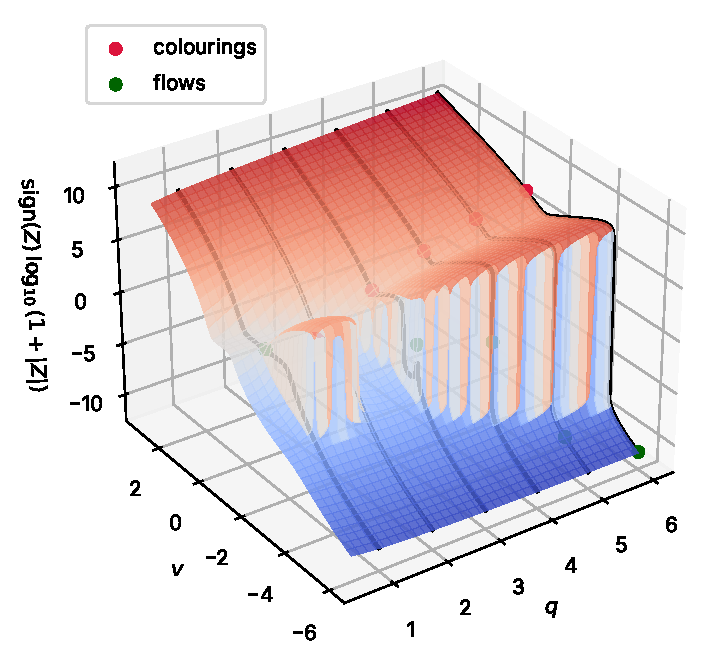
\includegraphics[width=0.78\textwidth]{figures/fig_tutte.pdf}
\caption{The random-cluster partition function $Z(G;q,v)$ of the Petersen graph
over the $(q,v)$-plane, as $\operatorname{sign}(Z)\log_{10}(1+|Z|)$, computed from
the $2^{15}$ edge subsets. Theorem~\ref{thm:tutte} evaluates it along the lines
$q=1,2,3,\dots$ drawn on the surface, which are the hyperbolas $H_q$ of the
Tutte plane; the marked points are the proper $q$-colourings ($v=-1$) and the
nowhere-zero flows ($v=-q$).}
\label{fig:tutte}
\end{figure}

\begin{remark}\label{rem:tutte}
Evaluating the Tutte polynomial is $\#$P-hard at every point of the plane
except on the hyperbola $H_1$ and at eight special points \cite{JVW90}; the
points of $H_q$ for positive integers $q$ include the chromatic and flow
polynomials at $q$, the Ising model ($q=2$) and the Potts models. On
bounded-degree graphs Theorem~\ref{thm:tutte} evaluates all of them in time
$2^{o(n)}$. The theorem does not evaluate $T$ off these hyperbolas: the number
of acyclic orientations $T(G;2,0)$, which lies on $H_{-1}$, the number of
forests $T(G;2,1)$ on $H_0$, and the reliability polynomial on $H_1$, trivial,
are not covered, and neither is the chromatic polynomial as a polynomial in $q$,
which would need the values at $n+1$ integers $q$ while the constant in the
exponent grows with $q$.
\end{remark}

\subsection{Linear codes with sparse parity checks}\label{ssec:codes}
A binary linear code of length $n$ given by a parity-check matrix
$H\in\Ftwo^{m\times n}$ is $\mathcal C=\{x\in\Ftwo^n:Hx=0\}$. Its weight
enumerator is the sequence $A_i=\#\{x\in\mathcal C:\operatorname{wt}(x)=i\}$,
$0\le i\le n$, where $\operatorname{wt}$ is the Hamming weight, and its minimum
distance is $d(\mathcal C)=\min\{i\ge1:A_i>0\}$. For a received word
$y\in\Ftwo^n$ the distance distribution of $y$ is
$A_i(y)=\#\{x\in\mathcal C:\operatorname{wt}(x+y)=i\}$, the weight enumerator of
the coset $y+\mathcal C$; a codeword at distance $\min\{i:A_i(y)>0\}$ from $y$ is a
maximum-likelihood decoding of $y$ on the binary symmetric channel. The codes
whose parity-check matrix has rows of bounded weight are the low-density
parity-check codes of Gallager \cite{Gal62}.

\begin{theorem}[Sparse parity checks]\label{thm:codes}
Fix $k,c\ge1$. Let $\mathcal C\subseteq\Ftwo^n$ be given by a parity-check matrix
with $m\le cn$ rows, each of weight at most $k$.
\begin{enumerate}[label=\textup{(\roman*)},leftmargin=2.2em]
\item\label{it:wenum} The weight enumerator $(A_i)_{0\le i\le n}$, and hence
$d(\mathcal C)$ and the number of minimum-weight codewords, are computed
deterministically in time $\poly(n)2^{O_{k,c}(\rhon(n))}$.
\item\label{it:coset} For every $y\in\Ftwo^n$ the distance distribution
$(A_i(y))_i$ is computed in the same time, and a codeword nearest to $y$ is
found in $2n+1$ times that time.
\item\label{it:qary} For a code over a finite field $\mathbb F_Q$, or over any
alphabet of fixed size $Q$ with the checks given as tables on $[Q]^{k}$, given by
$m\le cn$ checks each involving at most $k$ coordinates, the Hamming weight
enumerator and the distance distribution of every received word are computed
in time $\poly(n)2^{O_{Q,k,c}(\rhon(n))}$; so is the complete weight enumerator,
the number of codewords with $i_s$ coordinates equal to $s$ for each symbol
$s$, in time $\poly(n^{Q})2^{O_{Q,k,c}(\rhon(n))}$.
\end{enumerate}
\end{theorem}

\begin{proof}
\ref{it:wenum} Boolean variables $x_1,\dots,x_n$ and $\A=\A_{n+1}$. For each row
$h$ of $H$ take the multilinear extension of the indicator, on the scope
$\operatorname{supp}(h)$ of size at most $k$, that $\sum_{v\in\operatorname{supp}(h)}x_v$
is even; its coefficients are integers of absolute value at most $2^{k}$. For
each coordinate take $1+(W-1)Y_v$. There are at most $(c+1)n$ factors of scope at
most $k$, and the sum is $\sum_{x\in\mathcal C}W^{\operatorname{wt}(x)}=\sum_iA_iW^{i}$,
with no truncation. Theorem~\ref{thm:weighted} and Lemma~\ref{lem:bits} with
$N=n+1$, $L=k$ give the time; $d(\mathcal C)$ and $A_{d}$ are read off.

\ref{it:coset} Replace the coordinate factor by the multilinear extension of
$W^{[x_v\ne y_v]}$, which is $1+(W-1)Y_v$ if $y_v=0$ and $W+(1-W)Y_v$ if $y_v=1$;
the sum is $\sum_{x\in\mathcal C}W^{\operatorname{wt}(x+y)}=\sum_iA_i(y)W^{i}$. For
the nearest codeword let $i_0=\min\{i:A_i(y)>0\}$ and fix the coordinates one at
a time: fixing $x_1=\epsilon$ replaces every row containing coordinate $1$ by
the indicator that the remaining coordinates have parity $\epsilon h_1$, a
factor of smaller scope, and leaves the system sparse; compute the two distance
distributions, keep a value $\epsilon$ for which the coefficient of
$W^{i_0}$ is positive, and continue with the next coordinate. After $n$ steps the
assignment is a codeword at distance $i_0$ from $y$, and $2n+1$ distributions
have been computed.

\ref{it:qary} Apply Theorem~\ref{thm:domain} with $D=Q$: the variables take
values in the alphabet, each check is a table on at most $k$ coordinates, and
the coordinate factor has the table $s\mapsto W^{[s\ne0]}$, or
$s\mapsto W^{[s\ne y_v]}$ for the distance to $y$, in $\A_{n+1}$; for the
complete weight enumerator the table is $s\mapsto W_s$ in
$\A_{n+1,\dots,n+1}$ with one generator per symbol, of dimension $(n+1)^{Q}$.
\end{proof}

\begin{remark}
Computing the minimum distance of a binary linear code is NP-hard
\cite{Var97}, and so is maximum-likelihood decoding \cite{BMT78}; both are
posed with the code given by a generator or a parity-check matrix of
unrestricted density. For the low-density codes of Gallager, with $m\le n$ rows
of bounded weight, Theorem~\ref{thm:codes} gives the exact minimum distance, the
complete weight enumerator and exact maximum-likelihood decoding of every
received word in deterministic time $2^{o(n)}$, where the previously known
exact methods are exponential in the dimension or the redundancy of the code.
No bound on the column weights is needed, by Lemma~\ref{lem:frequent}.
\end{remark}

\subsection{Bounded-degree hypergraphs}\label{ssec:hypergraphs}
A hypergraph $\mathcal H=(V,\mathcal E)$ has vertex set $V$, $|V|=n$, and a
multiset $\mathcal E$ of edges $e\subseteq V$. A matching is a set of pairwise
disjoint edges, a perfect matching or exact cover is a matching whose union is
$V$, a transversal is a set of vertices meeting every edge, an independent set is
a set of vertices containing no edge, and a strong independent set is a set of
vertices no two of which lie in a common edge. A $q$-colouring of $V$ is proper
if no edge of size at least two is monochromatic.

\begin{theorem}[Hypergraphs]\label{thm:hypergraphs}
Fix $k,\Delta,c\ge1$ and $q\ge2$, and let $\mathcal H$ have $n$ vertices and
edges of size at most $k$.
\begin{enumerate}[label=\textup{(\roman*)},leftmargin=2.2em]
\item\label{it:hmatch} If every vertex lies in at most $\Delta$ edges and the
edges have integer weights in $[0,\Omega]$: the number of matchings of each
weight and the number of exact covers of each weight, hence the maximum weight
of a packing and the number of exact covers, in time
$\poly(n,\Omega)2^{O_{k,\Delta}(\rhon(n))}$.
\item\label{it:hindep} If $|\mathcal E|\le cn$ and the vertices have integer
weights in $[0,\Omega]$: the number of transversals, of independent sets and of
strong independent sets of each weight, in time
$\poly(n,\Omega)2^{O_{k,c}(\rhon(n))}$.
\item\label{it:hcol} If $|\mathcal E|\le cn$: the number of proper
$q$-colourings, and the number of $q$-colourings with exactly $j$ monochromatic
edges for every $j$, in time $\poly(n)2^{O_{q,k,c}(\rhon(n))}$.
\end{enumerate}
\end{theorem}

\begin{proof}
\ref{it:hmatch} A vertex in no edge lies in no exact cover and in every matching
trivially; delete such vertices, so that $n\le k|\mathcal E|$, and if
$|\mathcal E|<20$ list the subsets. Boolean variables $y_e$, $e\in\mathcal E$;
for each vertex $v$ the multilinear extension on the scope
$\{e:v\in e\}$, of size at most $\Delta$, of the indicator that at most one
(for matchings) or exactly one (for exact covers) incident edge is chosen; for
each edge $1+(W^{\omega_e}-1)Y_e$. There are $n+|\mathcal E|\le(k+1)|\mathcal E|$
factors of scope at most $\Delta$, the sum is
$\sum_M W^{\omega(M)}$ over the matchings, or over the exact covers, in $\A_N$
with $N=1+\sum_e\omega_e$, and Theorem~\ref{thm:weighted} on $|\mathcal E|\le\Delta n$
variables with the constants $\Delta$ and $k+1$, with Lemma~\ref{lem:bits},
$L=\Delta$, gives the bound; $\rhon(|\mathcal E|)=O_\Delta(\rhon(n))$.

\ref{it:hindep} Boolean variables $x_v$; for each edge $e$ the multilinear
extension, on the scope $e$, of the indicator that some $x_v$, $v\in e$, is $1$
(transversals), that not all are $1$ (independent sets), or that at most one
is $1$ (strong independent sets); for each vertex $1+(W^{\omega_v}-1)Y_v$. At most
$(c+1)n$ factors of scope at most $k$; Theorem~\ref{thm:weighted} and
Lemma~\ref{lem:bits} with $L=k$.

\ref{it:hcol} Theorem~\ref{thm:domainprofile} with $D=q$ and, for each edge of
size at least two, the constraint that it is monochromatic, of weight $1$: the
coefficient $p_j$ counts the colourings with $j$ monochromatic edges and $p_0$
the proper ones.
\end{proof}

\subsection{Circuits of linear size}\label{ssec:circuits}
A Boolean circuit with $n$ inputs is a sequence of gates $g_1,\dots,g_s$, each
computing a function of at most $k$ earlier gates or inputs given by its truth
table, with $t$ of the gates designated as outputs. Its size is $s$.

\begin{theorem}[Linear-size circuits of bounded fan-in]\label{thm:circuits}
Fix $k,c\ge1$. Let $C$ be a circuit with $n\ge20$ inputs, $s\le cn$ gates of
fan-in at most $k$, and outputs $o_1,\dots,o_t$ with integer weights
$\omega_1,\dots,\omega_t\in[0,\Omega]$. The numbers
\[
  N_{i,j}=\#\Bigl\{x\in\{0,1\}^n:\ \operatorname{wt}(x)=i,\ \sum_{l=1}^{t}\omega_l\,o_l(x)=j\Bigr\}
\]
are computed deterministically, for all $(i,j)$, in time
$\poly(n,\Omega)2^{O_{k,c}(\rhon(n))}$. In particular the number of inputs
accepted by a single-output circuit, and the maximum over the inputs of a
weighted sum of its output bits with the number of inputs attaining it, are
computed in that time.
\end{theorem}

\begin{proof}
Take the $n+s$ Boolean variables $x_1,\dots,x_n,g_1,\dots,g_s$ and
$\A=\A_{n+1,\,1+\sum_l\omega_l}$ with generators $U$ and $W$. For each gate $g$
take the multilinear extension, on the scope consisting of $g$ and its at most
$k$ arguments, of the indicator that $g$ equals the value of its function at the
arguments; for each input $1+(U-1)Y_{x_v}$; for each output $o_l$ the factor
$1+(W^{\omega_l}-1)Y_{o_l}$. There are $s+n+t\le(2c+1)n\le(2c+1)(n+s)$ factors of
scope at most $k+1$, with coefficients of absolute value at most $2^{k+1}$. For
each input $x$ exactly one assignment of the gate variables makes every gate
factor $1$, the one in which each $g$ carries its value at $x$, and every other
assignment makes some gate factor $0$; so the sum over the cube is
$\sum_xU^{\operatorname{wt}(x)}W^{\sum_l\omega_lo_l(x)}=\sum_{i,j}N_{i,j}U^{i}W^{j}$,
with nothing truncated. Theorem~\ref{thm:weighted} on $n+s\le(c+1)n$ variables
with the constants $k+1$ and $2c+1$, and Lemma~\ref{lem:bits} with $L=k+1$,
give the time, since $\rhon(n+s)\le\rhon((c+1)n)=O_c(\rhon(n))$.
\end{proof}

\begin{remark}
The count of the accepted inputs of a circuit with $s$ gates is, through the
Tseitin encoding used in the proof, the count of the satisfying assignments of a
$(k+1)$-CNF formula with $n+s$ variables, so for every $s$ it is contained in
\oai{}'s Theorem~1.1 with the exponent $o(n+s)$; their Corollary~1.4 draws a
circuit lower bound from exactly this fact. Theorem~\ref{thm:circuits} adds the
Hamming weight of the input and the weighted output profile for the sparse
case, which turns any objective computable by a linear-size circuit of bounded
fan-in on $n$ Boolean variables into one that is maximised exactly in time
$2^{o(n)}$, together with the number of maximisers. Theorems \ref{thm:profile},
\ref{thm:edges} and \ref{thm:codes} are instances, since their constraints are
computed by such circuits; the direct encodings given there avoid the gate
variables and have smaller constants.
\end{remark}

\subsection{Integer programs with sparse rows}\label{ssec:ip}
A $0$-$1$ integer program asks for a vector $x\in\{0,1\}^n$ satisfying a system
of linear inequalities and maximising a linear objective. Its rows need not
be clauses, cuts or parity checks: a row is an arbitrary linear form with
integer coefficients, compared with an integer by $\le$, $=$ or $\ge$. When
every row involves at most $k$ variables and there are $O(n)$ of them, each row
is a local constraint, and Theorem~\ref{thm:linear} adds a fixed number of
dense rows and the objective as linear statistics.

\begin{theorem}[Sparse integer programs]\label{thm:ip}
Fix integers $k,c\ge1$ and $s\ge0$. Consider $n\ge20$ variables, $m\le cn$
sparse rows
\[
  \sum_{v\in I_f}a_{f,v}x_v\ \bowtie_f\ b_f,\qquad |I_f|\le k,\quad
  {\bowtie_f}\in\{\le,=,\ge\},\quad a_{f,v},b_f\in\Z,
\]
with coefficients of arbitrary size, a cost vector $\gamma$ and dense rows
$\alpha^{(1)},\dots,\alpha^{(s)}$ in $\{-\Omega,\dots,\Omega\}^n$, $\Omega\ge1$,
and let $P\subseteq\{0,1\}^n$ be the set of vectors satisfying the sparse rows.
\begin{enumerate}[label=\textup{(\roman*)},leftmargin=2.2em]
\item\label{it:ip01} The numbers
\[
  p(j_0,\dots,j_s)=\#\bigl\{x\in P:\ \gamma\cdot x=j_0,\ \alpha^{(i)}\cdot x=j_i\ (1\le i\le s)\bigr\}
\]
are computed for all tuples in time
$\poly\bigl(\ell,(1+2n\Omega)^{s+2}\bigr)\,2^{O_{k,c,s}(\rhon(n))}$, where $\ell$
is the bit length of the input. Hence the largest and the smallest value of
$\gamma\cdot x$ over the $x\in P$ with $\alpha^{(i)}\cdot x\bowtie_i\beta_i$ for
prescribed relations $\bowtie_i$ and integers $\beta_i$, and the number of
vectors attaining each, are computed within the same time.
\item\label{it:ipD} For a fixed $D\ge1$ the same holds for vectors
$x\in\{0,1,\dots,D\}^n$, with time
$\poly\bigl(\ell,(1+4Dn\Omega)^{s+2}\bigr)\,2^{O_{D,k,c,s}(\rhon(n))}$.
\end{enumerate}
\end{theorem}

\begin{proof}
\ref{it:ip01} For each sparse row let $\phi_f:\{0,1\}^{I_f}\to\{0,1\}$ be the
indicator that the row holds, and let $\Phi_f$ be its multilinear extension
\eqref{eq:multilinear}. The table of $\phi_f$ has at most $2^k$ entries, each
found by one evaluation of the row, at a cost of $\poly(\ell)$ bit operations;
the coefficients of $\Phi_f$ are integers of absolute value at most $2^k$. So
$(\Phi_f)$ is a factor system with at most $cn$ factors of scope at most $k$
and values in $\Q$, and its product at $x\in\{0,1\}^n$ is the indicator of $P$.
To bring the statistics to nonnegative weights, put
$\omega^{(0)}_v=\gamma_v+\Omega$, $\omega^{(i)}_v=\alpha^{(i)}_v+\Omega$ for
$1\le i\le s$, and $\omega^{(s+1)}_v=1$, all in $[0,2\Omega]$. For every $x$,
\[
  \gamma\cdot x=\omega^{(0)}\cdot x-\Omega\,|x|,\qquad
  \alpha^{(i)}\cdot x=\omega^{(i)}\cdot x-\Omega\,|x|,\qquad |x|=\omega^{(s+1)}\cdot x .
\]
Theorem~\ref{thm:linear}\ref{it:lineq} with $N_0=1$, the $s+2$ weight vectors
$\omega^{(0)},\dots,\omega^{(s+1)}$ and the weight bound $2\Omega$ computes the
numbers $r(j'_0,\dots,j'_{s+1})$ of $x\in P$ with $\omega^{(i)}\cdot x=j'_i$ for
all $i$, in time $\poly(n,(1+2n\Omega)^{s+2})2^{O_{k,c,s}(\rhon(n))}$, to which
the cost $cn2^k\poly(\ell)$ of the tables is added. Then
\[
  p(j_0,\dots,j_s)=\sum_{t=0}^{n}r\bigl(j_0+\Omega t,\ j_1+\Omega t,\dots,\ j_s+\Omega t,\ t\bigr),
\]
because a vector with $|x|=t$ has $\omega^{(i)}\cdot x=\alpha^{(i)}\cdot x+\Omega t$.
The optimum over the $x\in P$ with $\alpha^{(i)}\cdot x\bowtie_i\beta_i$ is the
largest, or smallest, $j_0$ for which $\sum p(j_0,j_1,\dots,j_s)>0$, the sum
taken over the tuples with $j_i\bowtie_i\beta_i$, and that sum counts the
optimal vectors.

\ref{it:ipD} Let $T=\lceil\log_2(D+1)\rceil$ and replace each $x_v$ by $T$
Boolean variables $x_{v,0},\dots,x_{v,T-1}$ with $x_v=\sum_t2^tx_{v,t}$. A sparse
row becomes a sparse row in the new variables, with the coefficients
$2^ta_{f,v}$ and at most $kT$ variables; add for each $v$ the row
$\sum_t2^tx_{v,t}\le D$, which involves $T$ variables. The cost and the dense
rows become vectors with entries $2^t\gamma_v$ and $2^t\alpha^{(i)}_v$, of
absolute value at most $2^T\Omega\le2(D+1)\Omega\le4D\Omega$. The new program
has $n'=Tn$ variables and at most $(c+1)n\le(c+1)n'$ sparse rows of at most $kT$
variables, and its feasible vectors correspond bijectively to the vectors of
$\{0,\dots,D\}^n$ satisfying the original sparse rows, with the same values of
$\gamma\cdot x$ and $\alpha^{(i)}\cdot x$. Part \ref{it:ip01} applies, with
$\rhon(Tn)\le4T\rhon(n)$ for $n\ge T$.
\end{proof}

The theorem places no bound on the coefficients of the sparse rows, only on
their number of variables; the polynomial bound $\Omega$ is needed only for the
objective and the dense rows, which enter through the exponents of the
generators. Three classical problems that are NP-hard in the strong sense fall
under it.

\begin{corollary}\label{cor:ip}
Fix $k,c,s\ge1$. Each of the following is computed deterministically in time
$\poly(\ell,\Omega^{s+2})\,2^{O(\rhon(n))}$, where $\ell$ is the length of the
input, together with the number of optimal solutions, the implied constant
depending on $k,c,s$.
\begin{enumerate}[label=\textup{(\alph*)},leftmargin=2.2em]
\item\label{it:exactcover} For $n$ sets over a universe of at most $cn$
elements, each element lying in at most $k$ of the sets, with costs in
$[0,\Omega]$: the least cost of an exact cover, of a set cover and the largest
cost of a set packing. Exact cover by $3$-sets is NP-complete already when
every element lies in exactly three sets \cite{Gon85}.
\item\label{it:poknap} For $n$ items with values and $s$ weight vectors in
$[0,\Omega]$, capacities $B_1,\dots,B_s$ and a partial order given by at most
$cn$ relations $u\prec v$: the largest value of a set of items within the
capacities that contains, with each item, every item below it. For $s=1$ this
is the partially ordered knapsack problem, which is NP-complete in the strong
sense \cite{JN83}.
\item\label{it:exactsat} For a system of at most $cn$ linear equations
$\sum_{v\in I_f}a_{f,v}x_v=b_f$ with integer coefficients, $|I_f|\le k$, and a
cost vector in $[-\Omega,\Omega]^n$: the number of its $0$-$1$ solutions of
each cost, and the least and largest cost; in particular the number of
solutions of a $1$-in-$k$-SAT instance with at most $cn$ clauses, and its
solutions with the fewest true variables.
\end{enumerate}
\end{corollary}

\begin{proof}
\ref{it:exactcover} Take a variable for each set and, for each element, the
row $\sum_{S\ni e}x_S=1$, $\ge1$ or $\le1$; each row involves at most $k$
variables, and there are at most $cn$ rows. The cost is $\gamma$, with $s=0$.
\ref{it:poknap} Take a variable for each item, the row $x_v-x_u\le0$, which
says that $x_v=1$ forces $x_u=1$, for each relation $u\prec v$, and the weight
vectors as dense rows with $\beta_i=B_i$ and $\bowtie_i$ the relation $\le$;
the downward closure of the chosen set under the given relations is
equivalent to its closure under the order they generate. \ref{it:exactsat}
The equations are the sparse rows; for $1$-in-$k$-SAT a clause on the
literals $\ell_1,\dots,\ell_k$ is the equation $\sum_i\ell_i=1$, where a
negated literal $1-x_v$ moves the constant $1$ to the right side. All three
are Theorem~\ref{thm:ip}\ref{it:ip01}.
\end{proof}

\subsection{Growing density}\label{ssec:density}
Every statement so far fixes the ratio $c$ of factors to variables. The
parameters of Lemma~\ref{lem:params} do not depend on the degree ratio
$\kappa$, and the exponent of Theorem~\ref{thm:bounded-occ} is linear in it.
When $\kappa$ grows with $n$ it pays to let the parameters follow it: fewer
groups, and so a smaller $Q/R$ in the Taylor count, in exchange for a larger
share of the cost spent on one group. With the entropy bound of
Lemma~\ref{lem:entropy} in place of \eqref{eq:logCq}, this extends the
subexponential regime to every ratio $\kappa=o(\sqrt{\log n/\log\log n})$.

Throughout, $\lambda=\lceil\log n\rceil$, $\nu=\lceil\log\lambda\rceil$, and
\[
  g(x)=x\,\bigl(\log(1/x)\bigr)^{3/2}\qquad(0<x<1),
\]
which is increasing on $(0,2^{-3}]$ and tends to $0$ with $x$.

\begin{theorem}[Bounded occurrences at a growing degree ratio]\label{thm:explicit}
There is an absolute constant $\lambda_0$ with the following property. Let $\A$
be a commutative $\Q$-algebra, and let a factor system on $n$ variables with
$\lambda\ge\lambda_0$ have largest scope $w\le\lambda^2$, largest occurrence
number $b\le\lambda^2-1$ and total degree $d\le an$, where $a\ge1$ is a
real number with
\[
  \theta:=a\sqrt{\nu/\lambda}\le2^{-15}.
\]
Then $Z$ in \eqref{eq:Z} is computed deterministically with at most
\begin{equation}\label{eq:explicit}
  |\F|\,\poly(n)\,2^{\,790\,n\,g(\theta)}
\end{equation}
operations in $\A$, evaluations of factors at inputs in $\Q[z]/(z^{J})$ with
$J\le n$, and bit operations on rational numbers, using polynomially many
elements of $\A$ and polynomially many bits of storage in addition to the
factors' own. The polynomial is absolute.
\end{theorem}

\begin{proof}
Adjoin the constant-one factors of Section~\ref{sec:design}, so that
\eqref{eq:nMb} holds with $b\le\lambda^2$ and $d$ unchanged. Replacing $a$ by
$\max(1,d/n)$, which is rational, computed from the input and not larger than $a$,
decreases $\theta$ and, as $g$ is increasing, the bound \eqref{eq:explicit}; so we
may assume $a=\max(1,d/n)$. Put
$L=\log(1/\theta)\ge15$ and choose
\[
  t=\lfloor L\rfloor,\quad r=2^{t},\quad Q=\Bigl\lfloor\frac{\lambda}{128t}\Bigr\rfloor,\quad
  R=32+\bigl\lceil16\sqrt{Q\nu}\,\bigr\rceil,\quad \tau=\frac1{r\lambda},\quad D=r^{2Q}.
\]
Thus $t$ is the largest integer with $4^ta^2\nu\le\lambda$, and $1/(2\theta)<r\le1/\theta$.
Since $a\ge1$ and $\lambda\le2^{\nu}$, $L\le\frac12\log(\lambda/\nu)\le\nu/2$, so
$t\le\nu/2$ and $r^2\le2^{\nu}\le2\lambda$.

We check the hypotheses of Lemma~\ref{lem:complete}. First, $\lambda\ge256t$, so
$Q\ge\lambda/(256t)$, and $\log D=2Qt\le\lambda/64$. Since $Q\nu\ge1$,
$R\le33+16\sqrt{Q\nu}\le49\sqrt{Q\nu}$, hence
\begin{equation}\label{eq:RQexplicit}
  \frac RQ\le49\sqrt{\frac\nu Q}\le784\sqrt{\frac{t\nu}{\lambda}}
  \le784\,\frac{\nu}{\sqrt{2\lambda}} ,
\end{equation}
which is at most $1/6$ once $\lambda\ge(6\cdot784)^2\nu^2/2$; so $R\ge32$, $6R\le Q$
and $R<Q$ for $\lambda\ge\lambda_0$. The balance conditions \eqref{eq:balance}
hold: $2(b+w)D^2\le4\lambda^2\,2^{\lambda/32}\le2^{\lambda-1}<n\le M$ and
$2Qr^2\le(\lambda/64t)\cdot2\lambda<n$ for $\lambda\ge\lambda_0$. For the interval
take $\mu=Q(r-1)/(2r)$, $A_0=\lfloor\mu-(R-1)/2\rfloor$ and
$\mathcal J=\{A_0,\dots,A_0+R-1\}$ as in the proof of Lemma~\ref{lem:params}; since
$R\le Q/6$ it lies in $\{0,\dots,Q\}$, and since $R\ge32$ it contains every integer
within $R/4$ of $\mu$. Hoeffding's inequality \eqref{eq:hoeffding} with $s=R/4$
and $R^2\ge256Q\nu$ gives
\[
  \Pr\Bigl[\Bin\Bigl(Q,\tfrac{r-1}{2r}\Bigr)\notin\mathcal J\Bigr]\le2e^{-R^2/(8Q)}
  \le2e^{-32\nu}\le2^{-4\nu}\le\frac1{r^2\,b\,\lambda}=\frac{\tau}{rb},
\]
because $r^2\le2^{\nu}$, $b\le\lambda^2\le2^{2\nu}$ and $\lambda\le2^{\nu}$. This is
\eqref{eq:tailreq}, and $0<\tau\le1/2$. Lemma~\ref{lem:complete} constructs the
design in polynomial time.

Now the costs of Proposition~\ref{prop:routine}. By \eqref{eq:degbound} with
$d\le an$, $q=\lfloor dR/Q\rfloor\le\chi n$ with $\chi=aR/Q$. Since
$\sqrt{\nu/\lambda}=\theta/a\le\theta$ and $t\le L$, \eqref{eq:RQexplicit} gives
\[
  \chi\le784\,a\sqrt{\frac{t\nu}{\lambda}}\le784\,\theta\sqrt L=:\bar\chi ,
\]
and $\bar\chi\le784\cdot2^{-15}\sqrt{15}<\frac1{10}$ because $x\sqrt{\log(1/x)}$
increases on $(0,2^{-15}]$. In particular $q\le n/2$ and $J=q+1\le n$.
Lemma~\ref{lem:entropy} and the monotonicity of $x\log(2en/x)$ in $x\le n$ give
\[
  \log C_q\le\bar\chi n\log\frac{2e}{\bar\chi}
  =784\,\theta\sqrt L\,n\Bigl(L+\log\frac{2e}{784\sqrt L}\Bigr)\le784\,n\,\theta L^{3/2}
  =784\,n\,g(\theta).
\]
The measurement count contributes
$2\tau n\log(2D+1)\le\frac{2n}{r\lambda}\bigl(\frac\lambda{64}+2\bigr)\le\frac nr$
and one group $\frac{2n}r$, together $\frac{3n}{r}<6n\theta\le6\,n\,g(\theta)$.
The logarithm of \eqref{eq:routinecost} is therefore at most
$\log(2Qr)+790\,n\,g(\theta)$. Each vector costs at most $|\F|$ factor evaluations
and a number of further operations polynomial in $n$, $|\F|$, $D$, $Q$, $R$, $J$,
$r$ and $M\le\lambda^2 n$, all of which are bounded by powers of $n$ and $|\F|$
since $D\le2^{\lambda/64}\le2n^{1/64}$. The storage bound is that of
Proposition~\ref{prop:routine}.

The parameters are computed from $n$ and $d$ with integer square roots and
exact rational comparisons, in $\poly(\log n,\log d)$ bit operations,
and the conditions of Lemma~\ref{lem:complete} are checked exactly as in the proof
of Lemma~\ref{lem:params}; the estimates above show that every check passes.
\end{proof}

For a fixed ratio $a$ one has $\theta=a\sqrt{\nu/\lambda}$ and $\log(1/\theta)\le\nu/2$,
so $g(\theta)\le a\nu^2/(2\sqrt{2\lambda})$, and \eqref{eq:explicit} is the bound of
Theorem~\ref{thm:bounded-occ} with $\beta=2$ up to the constant. The gain is in the
dependence on $a$: the exponent of Theorem~\ref{thm:bounded-occ} is
$a\,n\nu^2/\sqrt\lambda$, which is $o(n)$ only for $a=o(\sqrt\lambda/\nu^2)$, while
$n\,g(\theta)$ is $o(n)$ for every $a=o(\sqrt{\lambda/\nu})$. Two changes produce the
gain. The entropy bound \eqref{eq:Cqentropy} charges the Taylor count
$\log C_q\approx q\log(n/q)$, whereas \eqref{eq:logCq} charges $q\log(Q/R)$, larger by
the factor $\log(Q/R)/\log(Q/(aR))$, which grows with $a$. And the number of groups
$r=2^{\lfloor\log(1/\theta)\rfloor}$ shrinks as $a$ grows, which makes $Q$ larger and
$R/Q$ smaller at the price of the cost $3n/r$ of the groups, balanced against the
Taylor count.

\begin{theorem}[Growing density]\label{thm:density}
There are absolute constants $n_1$ and $\theta_1>0$ with the following property.
Let $n\ge n_1$, let $k\ge1$ be an integer and $c\ge1$ a real number with
\[
  \theta_n:=ck\sqrt{\frac{\log\log n}{\log n}}\le\theta_1,
\]
and let a factor system on $n$ variables have at most $cn$ factors, each of scope
at most $k$, with values in a commutative $\Q$-algebra $\A$. Then $Z$ in
\eqref{eq:Z} is computed deterministically with at most
\[
  \poly(n)\,2^{\,4800\,n\,g(\theta_n)}\ \le\ \poly(n)\,2^{\,1700\,ck\,\rhon(n)}
\]
operations in $\A$, evaluations of the factors at inputs in $\Q[z]/(z^{J})$,
$J\le n$, and bit operations on rationals, in polynomial space; the polynomial is
absolute. In particular the bound is $2^{o(n)}$ whenever
$ck=o\bigl(\sqrt{\log n/\log\log n}\bigr)$. If the coefficients of the factors are
polynomials in the generators of $\A=\A_N$ or $\A_{N_1,\dots,N_s}$ with integer
coefficients of at most $L$ bits, the bound holds for bit operations after
multiplication by a polynomial in $n$, $N$ and $L$.
\end{theorem}

\begin{proof}
Put $\theta_1=2^{-18}$ and $\varepsilon_n=\sqrt{\log\log n/\log n}$, so that
$\theta_n=ck\,\varepsilon_n\ge\varepsilon_n$. Let $n_1$ be so large that for
$n\ge n_1$ one has $\lambda-1\ge\lambda_0$, the absolute constant of
Theorem~\ref{thm:explicit}, and $\theta_1\sqrt{\log n/\log\log n}\le\lambda/2$, so
that $ck\le\lambda/2$. Apply Lemma~\ref{lem:frequent}: fewer than $2^{n/\lambda}$
assignments $y$, each leaving a system on $n'\ge n-n/\lambda\ge n/2$ variables with
$\lambda'=\lceil\log n'\rceil\in\{\lambda-1,\lambda\}$, $\nu'\le\nu$, scopes at most
$k\le\lambda'^2$, occurrence numbers at most $ck\lambda\le\lambda^2/2\le\lambda'^2-1$,
and total degree at most $kcn\le2ck\,n'$. Theorem~\ref{thm:explicit} applies with
$a=2ck$ and
\[
  \theta'=2ck\sqrt{\nu'/\lambda'}\le2ck\sqrt{2\nu/\lambda}\le6\,ck\,\varepsilon_n=6\theta_n\le2^{-15},
\]
where $\nu\le\log\log n+2\le3\log\log n$ and $\lambda\ge\log n$ were used for $n\ge20$.
As $g$ is increasing on $(0,2^{-3}]$,
$g(\theta')\le g(6\theta_n)\le6\theta_n\log^{3/2}(1/\theta_n)=6\,g(\theta_n)$.
Each $Z_y$ costs at most $cn\,\poly(n)\,2^{4740\,n\,g(\theta_n)}$ operations, and
$cn\le n^2$. The branching adds the factor $2^{n/\lambda}\le2^{n\varepsilon_n}\le2^{n\,g(\theta_n)}$,
since $1/\lambda\le1/\log n\le\varepsilon_n\le\theta_n$ and $\log(1/\theta_n)\ge18$. The total is
at most $\poly(n)2^{4741\,n\,g(\theta_n)}$, which gives the first bound. For the second,
$\log(1/\theta_n)\le\log(1/\varepsilon_n)\le\frac12\log\log n$, so
$g(\theta_n)\le ck\,\varepsilon_n(\log\log n)^{3/2}/2^{3/2}=ck\,\rhon(n)/(2^{3/2}n)$,
and $4800/2^{3/2}<1700$. If $ck=o(\sqrt{\log n/\log\log n})$ then $\theta_n\to0$ and
$g(\theta_n)\to0$. The space bound and $J\le n'\le n$ come from
Theorem~\ref{thm:explicit}, and the bit complexity is Lemma~\ref{lem:bits}: its
proof uses of the parameters only $Q,\lambda=O(\log n)$, $R<Q$ and $D\le2^{\lambda}$,
which hold here, and its polynomial depends on $|\F|\le n^2$ and $k\le\lambda^2$ only
through powers of $n$.
\end{proof}

The corollaries of Sections \ref{sec:applications} and \ref{sec:more} that are
proved by one application of Theorem~\ref{thm:weighted} to a factor system whose
number of factors is bounded by the number of constraints or edges of the input,
and whose scopes are bounded, therefore extend to inputs of growing density. For a
function $d(n)\ge1$ write
\[
  \delta_n=d(n)\sqrt{\frac{\log\log n}{\log n}} ;
\]
the condition $\delta_n\to0$ means $d(n)=o(\sqrt{\log n/\log\log n})$. We record the
two for which the question of the dense case was raised in the introduction.

\begin{corollary}[Cuts and spin systems at growing average degree]\label{cor:density}
Let $d=d(n)\ge1$ satisfy $\delta_n\to0$, and let $G$ be a graph with $n$ vertices and
at most $d(n)\,n$ edges.
\begin{enumerate}[label=(\roman*),leftmargin=2.2em]
\item\label{it:densecut} The cut profile $\bigl(\#\{S\subseteq V:|S|=i,\
e(S,V\setminus S)=j\}\bigr)_{i,j}$, in particular the maximum cut, the maximum
bisection and their numbers of optimal solutions, is computed in time
$\poly(n)\,2^{\,20000\,n\,g(\delta_n)}=2^{o(n)}$.
\item\label{it:denseising} The density of states of an Ising system on $G$
with integer couplings and fields, and that of the $q$-state Potts system on
$G$ for fixed $q$, are computed in time
$\poly(n,E_{\max})\,2^{\,O_q(n\,g(\delta_n))}=\poly(E_{\max})\,2^{o(n)}$.
\end{enumerate}
In particular the maximum cut and the ground-state energy of an Ising system on
a graph of average degree $d(n)$ are found in time $2^{o(n)}$ whenever
$d(n)=o(\sqrt{\log n/\log\log n})$.
\end{corollary}

\begin{proof}
\ref{it:densecut} The factor system of Corollary~\ref{cor:maxcut} has one factor
of scope $2$ per edge and one of scope $1$ per vertex, with values in
$\A_{n+1,\,m+1}$ and coefficients of absolute value at most $2$; so it has at
most $(d(n)+1)n\le2d(n)n$ factors of scope at most $2$. Theorem~\ref{thm:density}
with $k=2$ and $c=2d(n)$ applies once $4\delta_n\le\theta_1$, and gives
$\poly(n)2^{4800\,n\,g(4\delta_n)}$ operations; $g(4\delta_n)\le4g(\delta_n)$, and
Lemma~\ref{lem:bits} with $N=(n+1)(m+1)\le n^3$ and $L=1$ turns the count into the
time bound. The optimum and its multiplicity are read off the profile as in
Corollary~\ref{cor:maxcut}.
\ref{it:denseising} The factor system in the proof of Theorem~\ref{thm:ising}\ref{it:isingmodel}
has one factor of scope $2$ per edge and one of scope $1$ per vertex, with values
in $\A_N$, $N=2E_{\max}+1$, and coefficients of $O(\log E_{\max})$ bits; it has at
most $2d(n)n$ factors, and Theorem~\ref{thm:density} with $k=2$, $c=2d(n)$ and
Lemma~\ref{lem:bits} give the bound as in \ref{it:densecut}. The factor system
in the proof of Theorem~\ref{thm:ising}\ref{it:potts} lives on $n'=qn$ variables
and has $n$ factors of scope $q$ and at most $d(n)n$ of scope $2q$, with
coefficients of $O(q+\log E_{\max})$ bits; so it has at most
$(d(n)+1)n\le(d(n)+1)n'$ factors of scope at most $2q$. Theorem~\ref{thm:density}
on $n'$ variables with $k=2q$ and $c=d(n)+1$ has
$\theta_{n'}\le4q\,d(n)\sqrt{\log\log n'/\log n'}\le4q\,\delta_n$ for large $n$,
because $\log\log x/\log x$ decreases for $x\ge16$; it gives
$\poly(n)2^{4800\,qn\,g(4q\delta_n)}$ operations, and $g(4q\delta_n)\le4q\,g(\delta_n)$.
Lemma~\ref{lem:bits} turns the counts into time bounds, and the ground-state energy
and the partition functions follow as in Theorem~\ref{thm:ising}.
\end{proof}

At $d(n)=\sqrt{\log n}/(\log\log n)^3$, for instance, $\delta_n=(\log\log n)^{-5/2}$
and the exponent in \ref{it:densecut} is $O(n/(\log\log n)^2)$.

The cut function of a graph and that of its complement determine each other, so the
corollary also reaches graphs with $\Theta(n^2)$ edges whose complement is sparse.

\begin{corollary}[Graphs with sparse complements]\label{cor:complement}
Let $d=d(n)\ge1$ satisfy $\delta_n\to0$ and let $\Omega_0\ge1$ be an integer. Let
$H$ be a graph on a vertex set $V$ of size $n$ with at most $d(n)\,n$ edges, and let
$\omega$ be a weighting of the pairs of distinct vertices with $\omega_{uv}=\Omega_0$
for $uv\notin E(H)$ and $\omega_{uv}\in\{0,1,\dots,\Omega_0\}$ for $uv\in E(H)$. Then
the numbers
\[
  p_{i,j}=\#\Bigl\{S\subseteq V:\ |S|=i,\ \sum_{u\in S,\,v\notin S}\omega_{uv}=j\Bigr\}
\]
are computed for all $i,j$ in time $\poly(n,\Omega_0)\,2^{\,O(n\,g(\delta_n))}=\poly(\Omega_0)\,2^{o(n)}$.
In particular, for every graph $G$ on $n$ vertices whose complement has at most
$d(n)\,n$ edges, the cut profile of $G$, the maximum cut, the maximum and the
minimum bisection, and the numbers of optimal solutions, are computed in time
$2^{o(n)}$.
\end{corollary}

\begin{proof}
Put $\eta_{uv}=\Omega_0-\omega_{uv}\in\{0,\dots,\Omega_0\}$ for $uv\in E(H)$. Every pair
$\{u,v\}$ with $u\in S$ and $v\notin S$ carries the weight $\Omega_0$, less
$\eta_{uv}$ when it is an edge of $H$, and there are $|S|(n-|S|)$ such pairs; hence
\begin{equation}\label{eq:complementcut}
  \sum_{u\in S,\,v\notin S}\omega_{uv}=\Omega_0\,|S|\,(n-|S|)-\mathrm{cut}_\eta(S),
\end{equation}
where $\mathrm{cut}_\eta(S)$ is the total $\eta$-weight of the edges of $H$ between $S$
and $V\setminus S$. Corollary~\ref{cor:maxcut}, with Theorem~\ref{thm:density} in place
of Theorem~\ref{thm:weighted} as in the proof of Corollary~\ref{cor:density}\ref{it:densecut},
computes the numbers $q_{i,j}$ of sets $S$ of size $i$ with $\mathrm{cut}_\eta(S)=j$ in
the stated time; the algebra is $\A_{n+1,\,\Omega_0m+1}$ with $m=|E(H)|$, of dimension
polynomial in $n$ and $\Omega_0$. By \eqref{eq:complementcut},
$p_{i,j}=q_{i,\,\Omega_0i(n-i)-j}$, read as $0$ when the index is negative or exceeds
$\Omega_0 m$. For a graph $G$ take $H$ its complement, $\Omega_0=1$ and $\omega=0$ on
$E(H)$; then $\omega$ is the indicator of $E(G)$, and the maximum cut and the bisections
are read off the numbers $p_{i,j}$.
\end{proof}

Corollary~\ref{cor:complement} rests on the fact that the cut of the complete graph
depends on $|S|$ alone. More generally, the cut of a graph whose adjacency is a
fixed quadratic expression in a few vertex weights depends only on the values of
those weights on $S$, and these values are linear statistics in the sense of
Theorem~\ref{thm:linear}. A sparse perturbation of such a graph is then within reach.

\begin{theorem}[Sparse perturbations of graphs of bounded rank]\label{thm:lowrank}
Let $d=d(n)\ge1$ satisfy $\delta_n\to0$, and let $s\ge1$ and $\Omega\ge1$ be integers.
Let $V$ be a set of size $n$, let $w_1,\dots,w_s:V\to\{0,1,\dots,\Omega\}$ and let
$C=(c_{ab})$ be a symmetric $s\times s$ integer matrix with entries in
$[-\Omega,\Omega]$. Put
\[
  \omega_{uv}=\sum_{a,b=1}^{s}c_{ab}\,w_a(u)\,w_b(v)\qquad(u\ne v),
\]
let $H$ be a graph on $V$ with at most $d(n)\,n$ edges and let
$\eta:E(H)\to\{-\Omega,\dots,\Omega\}$, extended by $0$ to the other pairs. For
$S\subseteq V$ let $\mathrm{cut}(S)=\sum_{u\in S,\,v\notin S}(\omega_{uv}+\eta_{uv})$.
Then the numbers
\[
  p_{i,j}=\#\{S\subseteq V:\ |S|=i,\ \mathrm{cut}(S)=j\}\qquad(i\ge0,\ j\in\Z)
\]
are computed for all $i,j$ in deterministic time
\[
  \poly\bigl(n,\Omega,(1+n\Omega)^{s}\bigr)\,2^{\,O(n\,g(\delta_n))},
\]
which is $2^{o(n)}$ whenever $s\log(n\Omega)=o(n)$.
\end{theorem}

\begin{proof}
Encode $S$ by its indicator $x\in\{0,1\}^V$, and put $j_a=\sum_vw_a(v)x_v$ and
$\Sigma_a=\sum_vw_a(v)$. Every ordered pair $(u,v)$ with $u\in S$ and $v\notin S$
has $u\ne v$, so
\begin{equation}\label{eq:lowrankcut}
  \sum_{u\in S,\,v\notin S}\omega_{uv}
  =\sum_{a,b}c_{ab}\Bigl(\sum_{u\in S}w_a(u)\Bigr)\Bigl(\sum_{v\notin S}w_b(v)\Bigr)
  =\sum_{a,b}c_{ab}\,j_a(\Sigma_b-j_b)=:P(j_1,\dots,j_s),
\end{equation}
and $\mathrm{cut}(S)=P(j_1,\dots,j_s)+\mathrm{cut}_{\eta^+}(S)-\mathrm{cut}_{\eta^-}(S)$,
where $\eta^{\pm}=\max(\pm\eta,0)$ and $\mathrm{cut}_{\eta^\pm}(S)$ is the
$\eta^\pm$-weight of the edges of $H$ between $S$ and $V\setminus S$. Let
$N_\pm=1+\sum_e\eta^\pm_e\le1+d(n)n\Omega$, $N_a=1+\Sigma_a\le1+n\Omega$, and
\[
  \A=\Q[W_+,W_-,U,T_1,\dots,T_s]\big/\bigl(W_+^{N_+},W_-^{N_-},U^{n+1},T_1^{N_1},\dots,T_s^{N_s}\bigr),
\]
of dimension $N\le(1+d(n)n\Omega)^2(n+1)(1+n\Omega)^s$. For an edge $e=\{u,v\}$ of $H$
take the factor $1+(W_+^{\eta^+_e}W_-^{\eta^-_e}-1)(Y_u+Y_v-2Y_uY_v)$, the multilinear
extension of $W_+^{\eta^+_e[x_u\ne x_v]}W_-^{\eta^-_e[x_u\ne x_v]}$, and for a vertex $v$
the factor $1+(U\,T_1^{w_1(v)}\cdots T_s^{w_s(v)}-1)Y_v$, of degree one in $Y_v$ as in
the proof of Theorem~\ref{thm:linear}. There are at most $(d(n)+1)n\le2d(n)n$ factors
of scope at most $2$, with coefficients that are polynomials in the generators with
integer coefficients of absolute value at most $2$, and their sum is
\[
  Z=\sum_xW_+^{\mathrm{cut}_{\eta^+}(x)}W_-^{\mathrm{cut}_{\eta^-}(x)}U^{|x|}T_1^{j_1}\cdots T_s^{j_s}
  =\sum r(h_+,h_-,i,j_1,\dots,j_s)\,W_+^{h_+}W_-^{h_-}U^{i}T_1^{j_1}\cdots T_s^{j_s},
\]
with no term truncated. Theorem~\ref{thm:density} with $c=2d(n)$ and $k=2$ applies
once $4\delta_n\le\theta_1$ and computes $Z$ with $\poly(n)2^{4800\,n\,g(4\delta_n)}$
operations in $\A$, and $g(4\delta_n)\le4g(\delta_n)$; the bit bound of that theorem
gives the stated time. Finally
$p_{i,j}=\sum r(h_+,h_-,i,j_1,\dots,j_s)$ over the tuples with
$h_+-h_-+P(j_1,\dots,j_s)=j$, a sum over at most $N$ coefficients.
\end{proof}

\begin{corollary}[Blow-ups with few changes]\label{cor:blowup}
Let $d=d(n)$ satisfy $\delta_n\to0$ and let $s=s(n)=o(n/\log n)$. Let $F$ be a graph
on $\{1,\dots,s\}$, loops allowed, and let $V=V_1\cup\dots\cup V_s$ be a partition of a
set of size $n$. The blow-up $F[V_1,\dots,V_s]$ joins $u\in V_a$ and $v\in V_b$,
$u\ne v$, exactly when $ab\in E(F)$. For every graph $G$ on $V$ that differs from
the blow-up in at most $d(n)\,n$ pairs, the cut profile of $G$, its maximum cut, its
maximum and minimum bisection, and the numbers of optimal solutions, are computed in
time $2^{o(n)}$. This holds in particular for every graph that differs in at most
$d(n)\,n$ pairs from a complete multipartite graph with $o(n/\log n)$ parts.
\end{corollary}

\begin{proof}
Take $\Omega=1$, $w_a$ the indicator of $V_a$ and $c_{ab}=1$ for $ab\in E(F)$ and $0$
otherwise; then $\omega_{uv}$ is the adjacency of the blow-up, since exactly one
term of the sum is nonzero. Let $H$ be the graph of the pairs where $G$ and the
blow-up differ, with $\eta=+1$ on the pairs that are edges of $G$ only and $\eta=-1$ on
the others; then $\omega+\eta$ is the adjacency of $G$. Theorem~\ref{thm:lowrank} applies
with $s\log(n+1)=o(n)$, and the optima are read off the numbers $p_{i,j}$ as in
Corollary~\ref{cor:maxcut}.
\end{proof}

Corollary~\ref{cor:complement} is the case $s=1$, $w_1=1$, $c_{11}=\Omega_0$ of the
theorem. Without the perturbation the cut is the polynomial $P$ of the linear statistics
$j_a$, and its maximisation needs no part of the routine: the $s$-tuples $(j_a)$ that occur
are counted in time $\poly(n\Omega)^s$ by dynamic programming over the vertices, and
for a positive semidefinite objective of fixed rank Allemand, Fukuda, Liebling and
Steiner \cite{AFLS01} solve unconstrained $0$-$1$ quadratic optimisation in polynomial
time. The perturbation $\eta$ is what requires Theorem~\ref{thm:density}: for $s=1$ and
$\omega=0$ it is Max-Cut on a graph of average degree $d(n)$.

\begin{remark}\label{rem:lowrankcount}
The graphs reached by Theorem~\ref{thm:lowrank} in time $2^{o(n)}$ form a vanishingly
small part of all graphs. Fix $\varepsilon>0$ and parameters with
$s\log(n\Omega)\le\varepsilon n$. A graph $G$ covered by the theorem is determined by
$w_1,\dots,w_s$, $C$, the edge set of $H$ and the restriction of the adjacency of $G$ to
$E(H)$, since $\eta$ is then the difference of that restriction and $\omega$. There
are at most
\[
  (\Omega+1)^{ns}(2\Omega+1)^{s^2}\,n^{2d(n)n}\,2^{d(n)n}
\]
such choices. Because $s\le n$, both $ns\log(\Omega+1)$ and $s^2\log(2\Omega+1)$ are at
most $2n\,s\log(n\Omega)\le2\varepsilon n^2$, and $d(n)n(2\log n+1)=o(n^2)$, so the count
is at most $2^{5\varepsilon n^2}$ for $n$ large, while there are $2^{n(n-1)/2}$ graphs on
$V$. As $\varepsilon$ is arbitrary, the proportion of graphs on $V$ covered by the
theorem with parameters for which its bound is $2^{o(n)}$ tends to $0$, and the random
graph $G(n,\frac12)$ is covered with probability tending to $0$. The exact maximum cut
of every graph in time $2^{o(n)}$ is therefore not a consequence of the theorem, and it
is not proved in this paper.
\end{remark}

The bookkeeping of Corollary~\ref{cor:complement} applies as well to the profiles of Theorem~\ref{thm:profile} and
to the programs of Theorem~\ref{thm:ip}.

\begin{corollary}[Max-$k$-SAT and integer programs at growing density]\label{cor:densitysat}
Let $d=d(n)\ge1$ satisfy $\delta_n\to0$, and fix $k\ge1$ and $s\ge0$.
\begin{enumerate}[label=(\roman*),leftmargin=2.2em]
\item\label{it:densesat} For a $k$-CNF formula with $n$ variables and at most
$d(n)\,n$ clauses with integer weights in $[0,\Omega]$, the profile
\eqref{eq:csprofile}, and with it the maximum satisfiable weight and the
number of assignments attaining it, is computed in time
$\poly(n,\Omega)\,2^{O_k(n\,g(\delta_n))}=\poly(\Omega)\,2^{o(n)}$.
\item\label{it:denseip} For a program as in Theorem~\ref{thm:ip} with at most
$d(n)\,n$ sparse rows, each involving at most $k$ variables, the numbers
$p(j_0,\dots,j_s)$ of Theorem~\ref{thm:ip}\ref{it:ip01} are computed in time
$\poly\bigl(\ell,(1+2n\Omega)^{s+2}\bigr)\,2^{O_{k}(n\,g(\delta_n))}$.
\end{enumerate}
\end{corollary}

\begin{proof}
\ref{it:densesat} The factor system of the proof of Theorem~\ref{thm:profile}
has at most $d(n)n$ factors of scope at most $k$, with values in $\A_N$,
$N=1+\sum_f\omega_f\le1+d(n)n\Omega$, and coefficients of at most $k$ bits.
Theorem~\ref{thm:density} with $c=d(n)$ applies once $k\delta_n\le\theta_1$ and gives
$\poly(n)2^{4800\,n\,g(k\delta_n)}$ operations, with $g(k\delta_n)\le k\,g(\delta_n)$;
Lemma~\ref{lem:bits} gives the time bound.
\ref{it:denseip} The factor system of the proof of Theorem~\ref{thm:ip}, through
that of Theorem~\ref{thm:linear}, consists of the at most $d(n)n$ indicator
factors of the sparse rows and the $n$ factors $\Psi_v$ of scope $1$, at most
$2d(n)n$ factors of scope at most $k$, with values in an algebra of dimension
at most $(1+2n\Omega)^{s+2}$ and coefficients of at most $k+1$ bits.
Theorem~\ref{thm:density} with $c=2d(n)$ and Lemma~\ref{lem:bits} compute its
sum, and the numbers $p(j_0,\dots,j_s)$ are read off as in the proof of
Theorem~\ref{thm:ip}.
\end{proof}

\begin{remark}\label{rem:densityend}
The regime of Theorem~\ref{thm:density} ends at $ck$ of order
$\sqrt{\log n/\log\log n}$. Below that order the exponent is $o(n)$; at that order
$\theta_n$ is bounded away from $0$ and \eqref{eq:explicit} is no better than
enumeration. The routine of Proposition~\ref{prop:routine} cannot reach quadratic
density with any design at all. The balance condition \eqref{eq:balance} and
$M\le bn$ give $D^2\le M/(2(b+w))<n/2$, and $D=r^{2Q}\ge2^{2Q}$, so every admissible
design has $Q<\frac14\log n$. Consequently $q=\lfloor dR/Q\rfloor\ge\lfloor4d/\log n\rfloor$,
and $q\ge n$ as soon as the total degree satisfies $d\ge\frac14(n+1)\log n$; then
$C_q=\sum_{s=0}^n2^s\binom ns=3^n$, and the Taylor count \eqref{eq:Cq} alone is
exponential. For the cut factors $1+(W-1)(Y_u+Y_v-2Y_uY_v)$ of a graph with $m$ edges
the product over the edges has degree exactly $2m$ in the incidence indeterminates,
its top coefficient being $(-2)^m(W-1)^m\ne0$ in $\A_{m+1}$, so the degree bound
\eqref{eq:degbound} cannot be lowered and a graph with $m\ge\frac18(n+1)\log n$
edges already gives $q\ge n$. Branching on $h$ vertices costs $2^h$ and removes at
most $hn$ edges, so for a graph with $\Theta(n^2)$ edges any subexponential branching
leaves $\Theta(n^2)$ edges. This is a limitation of the routine, not a lower bound for
Max-Cut. The theorem is nonetheless a bound of the form $2^{o(n)}$ for the exact
maximum cut on graphs whose average degree tends to infinity, and
Corollary~\ref{cor:complement} and Theorem~\ref{thm:lowrank} give one for classes of
graphs with $\Theta(n^2)$ edges, though not for almost every graph
(Remark~\ref{rem:lowrankcount}); the algorithm of Williams \cite{Wil05} runs in time $2^{\omega n/3}$ on every
graph, and under the exponential time hypothesis no bound $2^{o(n)}$ was possible
even at bounded degree.
\end{remark}
